\section{Superfícies}



\noindent\textbf{{\large Superfícies Cilíndricas}}

Uma \dt{superfície cilíndrica} é aquela gerada por uma reta $\ell$ que se move ao longo de uma curva plana dada, de modo que a reta $\ell$ sempre esteja paralela a uma reta fixa. A reta $\ell$ é chada de \dt{geratriz} e a curva de \dt{diretriz}.

\begin{exeb}{}{}
	A equação $z=x^2$ em $\R^3$ representa a seguinte superfície cilíndrica.
	
	\begin{center}
		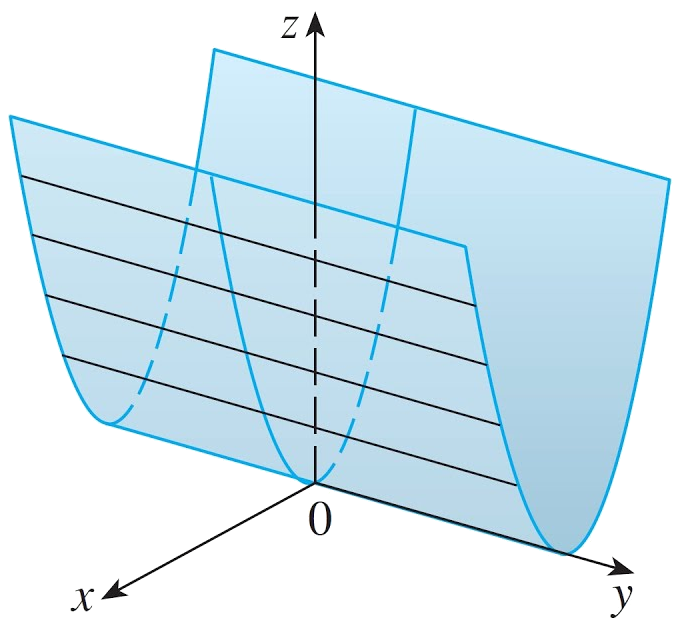
\includegraphics[scale=1]{figuras/cilindro-ex1.png}
	\end{center}
\end{exeb}

\begin{exeb}{}{}
Esboce as superfícies
	\begin{enumerate}[(a)]
		\item $y^2+z^2=1$
		\item $z=1-y^2$
	\end{enumerate}
\end{exeb}
\newpage

\noindent\textbf{{\large Superfícies Quádricas}}

Uma \dt{superfície quádrica} é o gráfico de uma equação do segundo grau a três variáveis, isto é, uma equação da forma:
\begin{equation*}
	{\color{red}A}x^2+{\color{red}B}y^2+{\color{red}C}x^2+{\color{red}D}xy
	+{\color{red}E}xz+{\color{red}F}yz+{\color{red}G}x+{\color{red}H}y+
	{\color{red}I}z+{\color{red}J}=0,
\end{equation*}
onde pelo menos um dos coeficientes ${\color{red}A}, {\color{red}B}, 
{\color{red}C}, {\color{red}D}, {\color{red}E}$ ou ${\color{red}F}$ é {\color{blue} não nulo}.

\begin{minipage}{0.5\textwidth}
	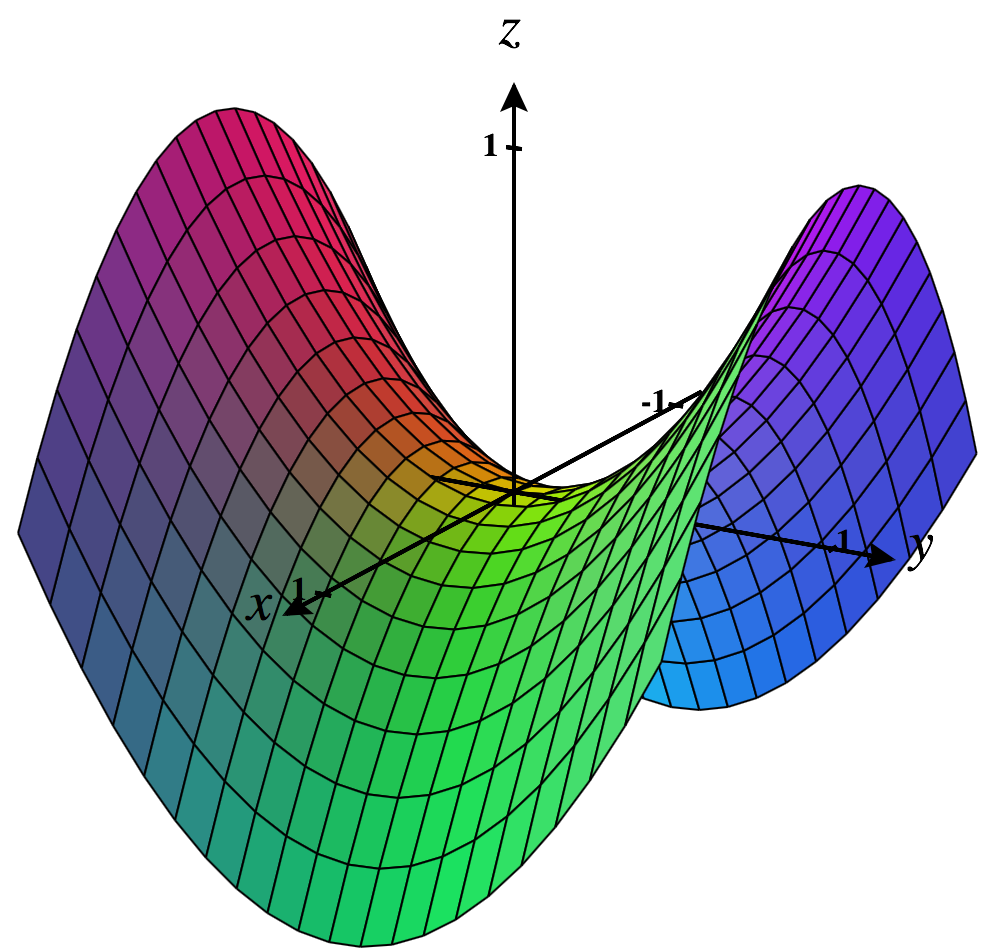
\includegraphics[scale=0.13]{figuras/quadricas/parab-hip.png}
\end{minipage}
\begin{minipage}{0.4\textwidth}
	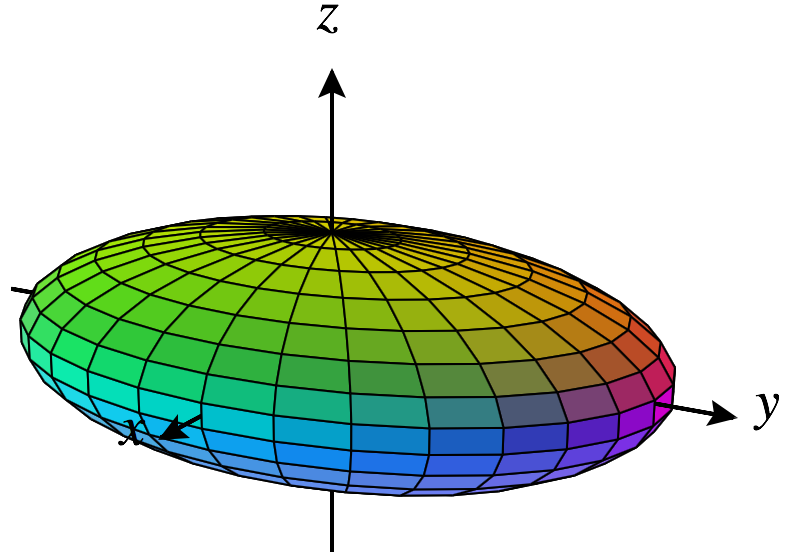
\includegraphics[scale=0.8]{figuras/quadricas/elipsoide.png}
\end{minipage}
\bigskip

\noindent\textbf{Forma Padrão}

Através de uma rotação e uma translação é possível colocar a {\color{blue}superfície quádrica} em uma das chamadas {\color{blue} formas padrão}.

\begin{center}
	\textbf{Elipsoide:} \(\frac{x^2}{a^2}+\frac{y^2}{b^2}+\frac{z^2}{c^2}=1\)
	\bigskip
	
	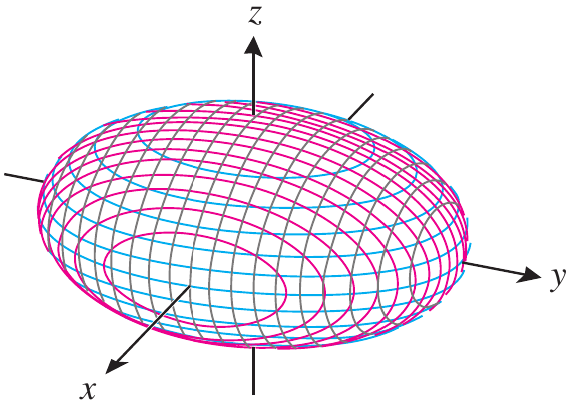
\includegraphics[scale=0.5]{figuras/quadricas/elipsoide-padrao.png}
\end{center}

\hrulefill


\begin{center}
	\textbf{Hiperboloide de uma folha:} \(\frac{x^2}{a^2}+\frac{y^2}{b^2}-\frac{z^2}{c^2}=1\)
	\bigskip
	
	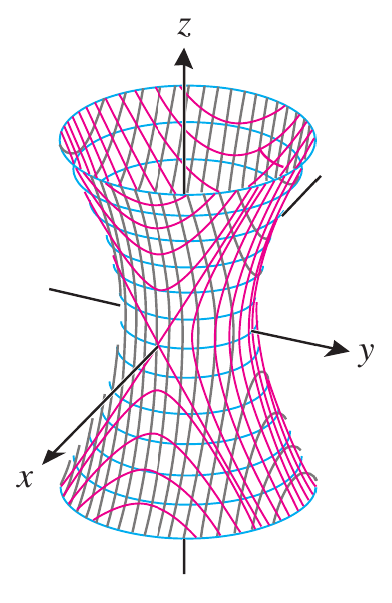
\includegraphics[scale=0.5]{figuras/quadricas/hiperboloide1-padrao.png}
\end{center}

\hrulefill

\begin{center}
	\textbf{Hiperboloide de duas folha:} \(-\frac{x^2}{a^2}-\frac{y^2}{b^2}+\frac{z^2}{c^2}=1\)
	\bigskip
	
	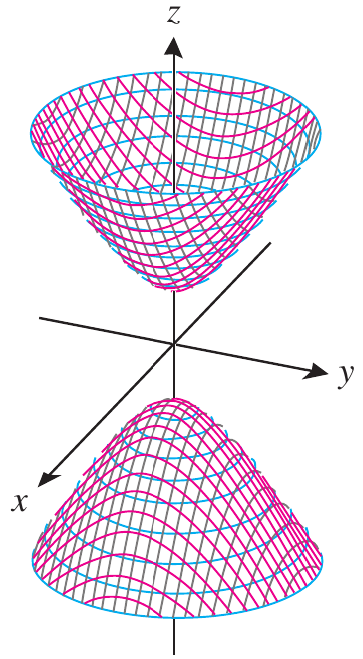
\includegraphics[scale=0.5]{figuras/quadricas/hiperboloide2-padrao.png}
\end{center}

\hrulefill

\begin{center}
	\textbf{Cone:} \(z^2=\frac{x^2}{a^2}+\frac{y^2}{b^2}\)
	\bigskip
	
	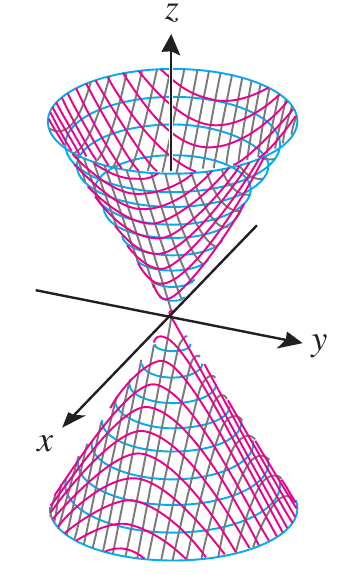
\includegraphics[scale=0.5]{figuras/quadricas/cone-padrao.png}
\end{center}

\hrulefill

\begin{center}
	\textbf{Paraboloide Elíptico:} \(z=\frac{x^2}{a^2}+\frac{y^2}{b^2}\)
	\bigskip
	
	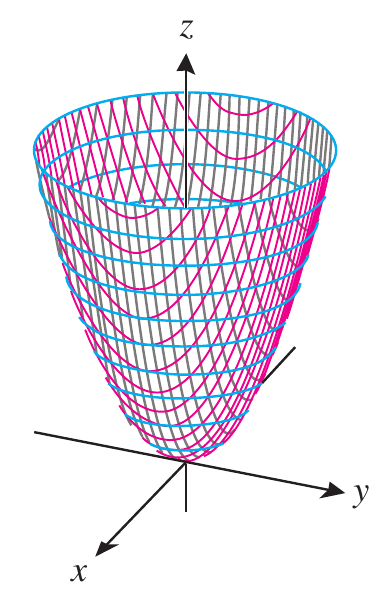
\includegraphics[scale=0.5]{figuras/quadricas/paraboloide-padrao.png}
\end{center}

\hrulefill

\begin{center}
	\textbf{Paraboloide Hiperbólico:} \(z=\frac{x^2}{a^2}-\frac{y^2}{b^2}\)
	\bigskip
	
	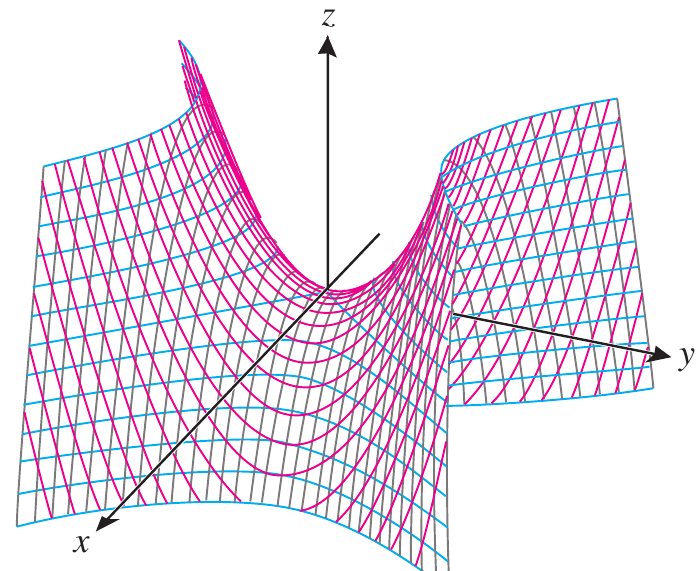
\includegraphics[scale=0.5]{figuras/quadricas/paraboloide-hiperbolico-padrao.png}
\end{center}

\begin{center}

\textbf{Resumo}

\begin{tabular}{|c|c|c|}
	\hline
	Equação & Característca  & Classifciação    \\
	\hline
	\(\frac{x^2}{a^2}+\frac{y^2}{b^2}+\frac{z^2}{c^2}=1\) & \makecell{3 termos quadráticos \(=1\) \\ Sem sinal negativo } & Elipsoide \linebreak    \\
	\hline
	\(\frac{x^2}{a^2}+\frac{y^2}{b^2}{\color{red}-}\frac{z^2}{c^2}=1\)& \makecell{3 termos quadráticos \(=1\) \\ {\color{red}1 sinal negativo} }  & \makecell{Hiperboloide \\ de {\color{red}  1 folha} }    \\
	\hline
	\({\color{red}-}\frac{x^2}{a^2}+\frac{y^2}{b^2}{\color{red}-}\frac{z^2}{c^2}=1\) & \makecell{3 termos quadráticos \(=1\) \\ {\color{red} 2 sinais negativo} }  & \makecell{Hiperboloide \\ de {\color{red} 2 folha} }    \\
	\hline
	\( \frac{x^2}{a^2}+\frac{y^2}{b^2}=\frac{z^2}{c^2} \)& \makecell{2 termos quadráticos  \\ \(=\) ao terceiro }
	& Cone   \\
	\hline
	\( {\color{blue} z}=\frac{x^2}{a^2}+\frac{y^2}{b^2} \)& \makecell{{\color{blue} 1 termo linear} \(=\) 2 
		quadráticos 
		\\ com mesmo sinal }   & \makecell{{\color{blue} Paraboloide}\\ Elíptico}   \\
	\hline
	\(  {\color{blue} z}=\frac{x^2}{a^2}-\frac{y^2}{b^2} \)& \makecell{{\color{blue} 1 termo linear} \(=\) 2 
		quadráticos 
		\\ com {\color{red} sinais opostos} }   & \makecell{ {\color{blue} Paraboloide}\\  {\color{red} Hiperbólico}}   \\
	\hline
\end{tabular}
\end{center}


\begin{exeb}{}{}
	Reconheça e esboce às quádricas
	\begin{enumerate}
		\item \(z=4x^2+y^2\)
		\item \(z=y^2-x^2\)
		\item \(\displaystyle\frac{x^2}{4}+y^2-\frac{z^2}{4}=1\)
	\end{enumerate}
\end{exeb}

